% doc/tikz/eci_ecef_frames.tex
\documentclass[tikz,border=5pt]{standalone}

\usepackage{amsmath, amssymb}
\usepackage{tikz}
\usetikzlibrary{
    arrows.meta,
    positioning,
    shapes.geometric,
    calc
}

\begin{document}
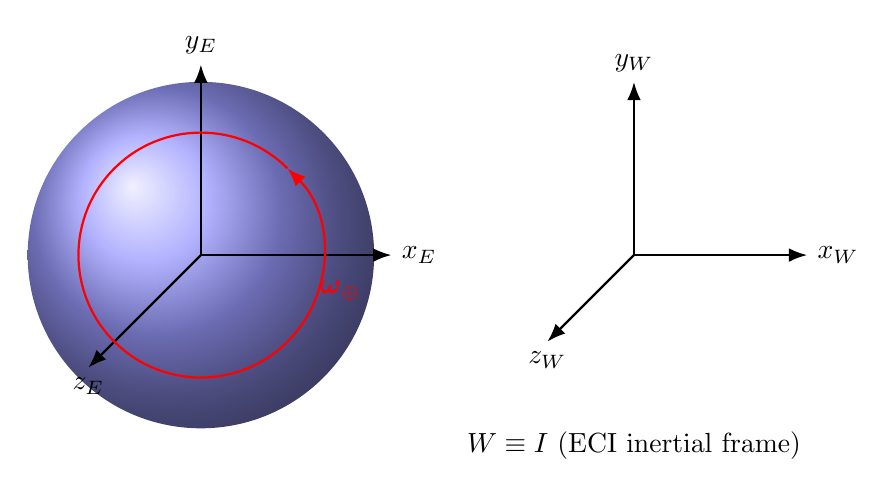
\begin{tikzpicture}[scale=1.1, >=Latex]

% Earth as a sphere
\shade[ball color=blue!40] (0,0) circle (2cm);

% ECEF axes
\draw[->, thick] (0,0) -- (2.2,0) node[right] {$x_E$};
\draw[->, thick] (0,0) -- (0,2.2) node[above] {$y_E$};
\draw[->, thick] (0,0) -- (-1.3,-1.3) node[below] {$z_E$};

% Earth rotation arrow
\draw[->, thick, red] (1,1) arc (45:405:1.414)
    node[pos=0.8, above right] {$\boldsymbol{\omega}_\oplus$};

% Inertial frame W (ECI) displaced to the right
\begin{scope}[shift={(5,0)}]
    \draw[->, thick] (0,0) -- (2,0) node[right] {$x_W$};
    \draw[->, thick] (0,0) -- (0,2) node[above] {$y_W$};
    \draw[->, thick] (0,0) -- (-1,-1) node[below] {$z_W$};
    \node at (0,-2.2) {$W \equiv I$ (ECI inertial frame)};
\end{scope}

\end{tikzpicture}
\end{document}
